\section{Задача автоматического выделения терминов: алгоритм TopMine, UDPipe, модель PLSA.}

Цель для такой задачи является выделение составных терминов в текстовых коллекциях. Термин - фраза (n-грамма) со следующим набором свойств:

\begin{itemize}
	\item Высокая частотность - много раз встречается в коллекции.
	\item Контактная сочетаемость слов - состоит из слов, неслучайно часто встречающихся вместе.
	\item Полнота - является максимальной по включению цепочкой слов.
	\item Синтактическая свяхность - является грамматически корректным словосочетанием.
	\item Тематичность - часто встречается в узком подмножестве тем.
\end{itemize}

Для проверки каждой из свойств используются 

\begin{itemize}
	\item Статистический анализ: для проверки первых трёх свойств терминов. Он позваляет находить высокочастотные токены, выделять слова, неслучайно стоящие рядом и штрафовать неполные последовательности слов, входящие как подмножество в другую высокочастотную последовательность неслучайно стоящих слов.
	\item Синтаксический анализ: для проверки синтактической связности. Данный анализ позволяет выделять синтактически связанные словосочетания в предложениях.
	\item Тематическая модель: для проверки тематичности. Она позволяет сопоставить каждому токену распределение тем.
\end{itemize}

Для каждого анализа мы будем использовать модели TopMine, UDPipe и PLSA для семантического, синтаксического анализа и тематической модели соответственно. Рассмотрим в подробности каждую модель

\subsection*{Статистический анализ: TopMine}

Этот алгоритм итеративно сливает слова и фразы в предложении, рассчитывая для каждого слияния оценку значимости \textit{SignificanceScore} и останавливается, когда для всех возможных слияний значимость меньше заданного порога. 

В начале мы должны найти все частые k-грамм и алгоритм быстрого поиска приведён на рисунке 1.
\begin{figure}
    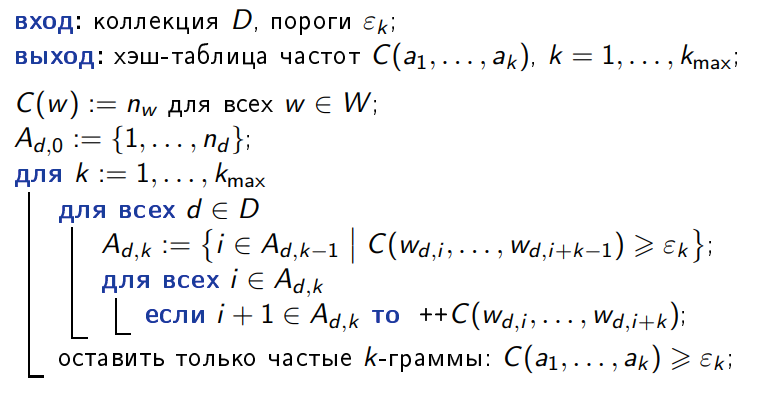
\includegraphics[scale = 0.5]{images/ml1.png}
    \caption{Алгоритм быстрого поиска}
\end{figure}
где $C(a_{1},...,a_{k})$ - хэш-таблица частот k-грамм, $a_{i} \in W$, $C(w) = n_{w}$ для всех униграмм $w \in W: n_{w} \geq \varepsilon_{1}$, где $W$ - множество слов или фраз.
$\varepsilon_{1}$ - пороговое значение частоты частых k-грамм
$A_{d,k}$ - множество позиций i в документе d, с которых начинаются все частые k-граммы
$C(w_{d,i},...,w_{d,i+k-1}) \geq \varepsilon_{k}$
Свойство антимонотонности: $C(a_{1},...,a_{k}) \geq C(a_{1},...,a{k+1})$

Затем должны провести итеративное слияние фраз с понижением значимости до $\alpha$.
$SignificanceScore = \frac{p_{uv}-p_{u}p_{v}}{\sqrt{p_{uv}}}$
где $p_{u}$ - оценка вероятности встретить фразу \textit{u}, $p_{uv}$ = оценка вероятности встретить фразу \textit{uv}.

В начале у нас есть кортеж исходных фраз и первой итерацией считается \textit{SignificanceScore} для всех соседних пар фраз. И затем из кортежа удаляются все все пары с \textit{SignificanceScore} больше $\alpha$. Оставшиеся элементы в кортеже и являются термами. На рисунке 2 приведен пример работы алгоритма TopMine.
\begin{figure}
    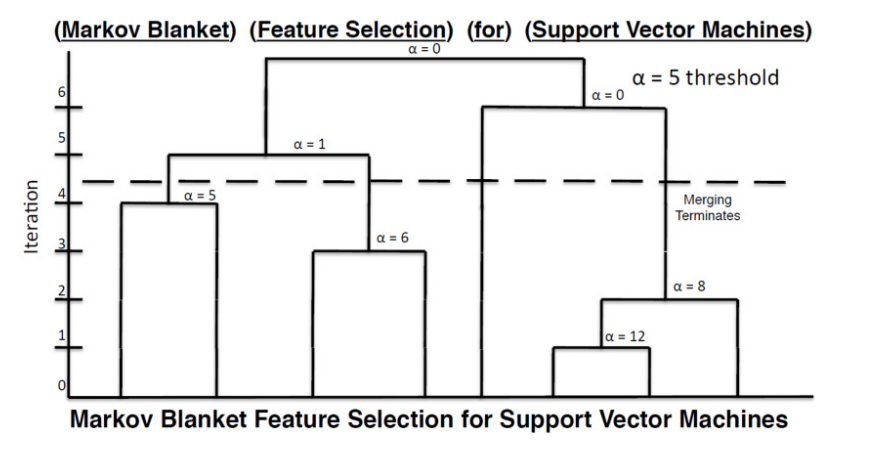
\includegraphics[scale = 0.5]{images/ml2.png}
    \caption{Пример работы алгоритма TopMine}
\end{figure}
\subsection*{Синтаксический анализ: UDPipe}

UDPipe - предобученная модель, которая может распозновать синтаксические связи в предложениях и разметка частей речи слов в предложениях. На вход подаётся список предложений, и для каждого слова в предложениях вычисляется:

\begin{itemize}
	\item Часть речи слова.
	\item Член предложения.
	\item ID родительского слова.
\end{itemize}

Модель для каждого предложения создаёт синтаксическое дерево, и при помощи неё проверяет словосочетании-кандидаты. Для них подсчитывается оценка его синтаксической связанности по формуле $SyntaxScore(W) = max SyntaxDistance(w_{i}, w_{j})$, где \textit{W} - N-грамма, $1 \leq i \leq N$, $1 \leq j \leq N$ и $i \neq j$.Таким образом, если одно из слов в словосочетании-кандидате синтактически не связанно с остальным, \textit{SyntaxScore} это выявит.

\subsection*{Тематический анализ: PLSA}

У нас есть коллекция текстовых документов $D$ и словарь токенов $W$, из которых состоят документы. Каждый документ $d \in D$ представляет собой последовательностью входящих в него токенов из словаря $W$. Если предположить, что местоположение токенов в документе не влияет на определение тематики документа, то документ это подмножество $d \subset W$, в котором каждому токену $w \in d$ поставлено в соответствие число $n_{dw}$ вхождений в документ $d$.

Модель описывает вероятности появления токенов $w$ в документов $d$ при предположении условной независимости:
$$p(w|d) = \sum_{t \in T} p(w|t)p(t|d) = \sum_{t \in T} \phi_{wt} \theta_{td}$$
где $\phi_{wt} = p(w|t), \theta_{td} = p(t|d)$ являются обучаемыми параметрами модели. Для обучения параметров модели, представленные в виде матрицы $\Phi = (\phi_{wt})_{WxT}$ и $\Theta = (\theta_{td})_{TxD}$ по коллекции документов $D$ максимизируется логарифм правдоподобия
$$L(\Phi, \Theta) = \sum_{d \in D} \sum_{w \in d} n_{dw} ln \sum_{t \in T} \phi_{wt} \theta_{td} \rightarrow \max_{\Phi, \Theta}$$

при ограничениях неотрицательности и нормировки
$$\sum_{w \in W} \phi_{wt} = 1, \phi_wt \geq 0, \sum_{t \in T} \theta_{td} = 1, \theta_{td} \geq 0$$

На основе полученных параметров $\Phi$ и $\Theta$ для каждого словосочетания-кандидата считается распределение тем $p(t|w) = \phi_{wt} \frac{p(t)}{p(w)}$. Отбор происходит распределением тематик $p(t|w)$ имеет высокую вероятность только для некоторых тем из малого подмножества всех тем T. Это можно оценить через отдаленность $p = p(t|w)$ от равномерного $p_{unif} = 1/T$, где $T$-мощьность множества $T$. Расстояние между двумя распределениями считается несколькими способами:

\begin{itemize}
	\item Дивергенция Кульбака-Лейблера
	$$KL(pp_{unif}) = \sum_{t \in T} \frac{1}{|T|} ln \frac{\frac{1}{|T|}}{p(t|w)}$$
	\item Дивергенция Йесена-Шеннона
	$$JS(pp_{unif}) = \frac{1}{2}KL(p_{unif}p_{1}) + \frac{1}{2}KL(pp_{1})$$
	$$p_{1}(t|w) = \frac{1}{2}(p(t|w) + \frac{1}{|T|})$$
	\item Сумма степенных функций, $\gamma > 1$
	$$Deg(p) = \sum_{t \in T} p(t|w)^{\gamma}$$
\end{itemize}

Чем больше значение данных метрик для $w$, тем тематичнее данная N-грамма.

\subsection*{Задачи}

\textbf{Задача 1.} Нам дана фраза \textit{a} \textit{b}, было оценено вероятность встречи фраз $p_{a} = 0,1$, $p_{b} = 0,2$, $p_{ab} = 0,05$. Пороговая значимость $\alpha = 1$. Является ли фраза \textit{ab} термином?

\textbf{Ответ:} Нет.

\textbf{Решение.} 
$$\frac{p_{ab}-p_{a}p_{b}}{\sqrt{p_{ab}}} \approx 0,01 < \alpha$$

 \textbf{Задача 2.} Дано синтактическое дерево (рис. 3) для предложения "An inventory of syntactic functions is taken to be primitive". Найдите \textit{SyntaxScore} для фразы "syntactic functions is".
 
\begin{figure}
    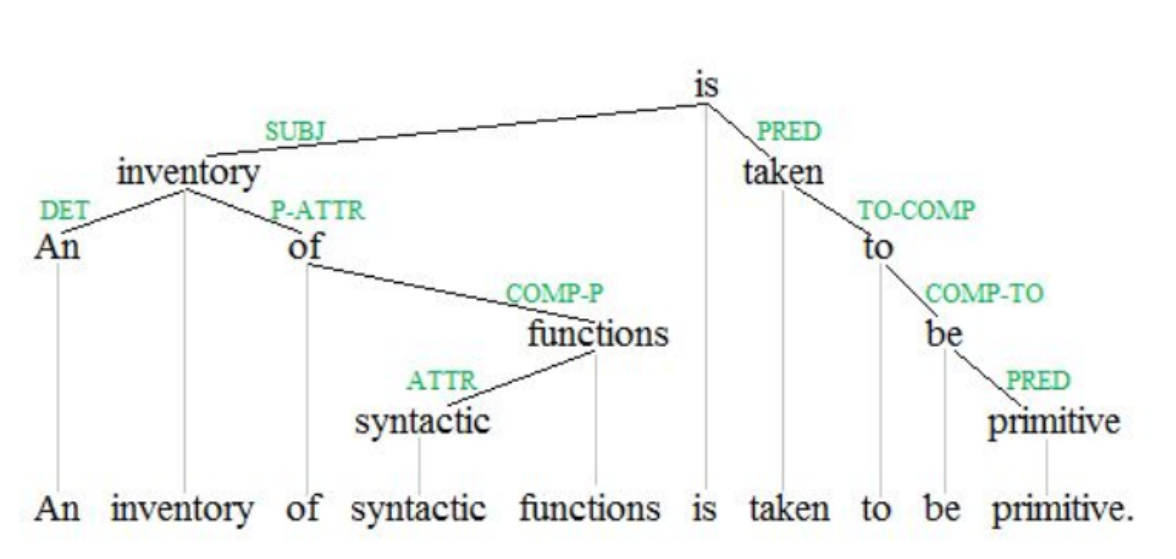
\includegraphics[scale = 0.4]{images/ml3.png}
    \caption{Задача 2}
\end{figure}

\textbf{Ответ:} 4.

\textbf{Задача 3.} Привести аналитическое решение максимизации задачи

$$L(\Phi, \Theta) = \sum_{d \in D} \sum_{w \in d} n_{dw} ln \sum_{t \in T} \phi_{wt} \theta_{td} \rightarrow \max_{\Phi, \Theta}$$

и выразить элементы матрицы $\Phi$ и $\Theta$ через $n_{dw}$ и $p(t|d,w)$.

\textbf{Решение.}

Запишем лангранжиан задачи, учитывая ограничение нормировки:

$$L(\Phi, \Theta) = \sum_{d \in D} \sum_{w \in d} n_{dw} ln \sum_{t \in T} \phi_{wt} \theta_{td} - \sum_{t \in T} \lambda_{t} (\sum_{w \in d} \phi_{wt} - 1) - \sum_{d \in D} \mu_{d} (\sum_{t \in T} \theta_{td} - 1)$$

Продифференцируем лангранжиан по $\phi_{wt}$ и приравняем к нулю производную, получим:

$$\lambda_{t} = \sum_{d \in D} n_{ds} \frac{\theta_{td}}{p(w|d)}$$

Домножив обе части на $\phi_{wt}$, получим:

$$\lambda_{t} \phi_{wt} = \sum_{d \in D} n_{ds} \frac{\phi_{wt} \theta_{td}}{p(w|d)}$$

По формуле Байеса:

$$p(t|d,w) = \frac{p(w|t) p(t|d)}{p(w|d)} = \frac{\phi_{wt} \theta_{td}}{p(w|d)}$$

Сделав замену  получим:

$$\lambda_{t} \phi_{wt} = \sum_{d \in D} n_{ds} p(t|d,w)$$

Просуммируем по $w \in W$ и получим:

$$\lambda_{t} \sum_{w \in W} \phi_{wt} = \sum_{w \in W} \sum_{d \in D} n_{ds} p(t|d,w)$$

В соответствии с условием нормировки $\sum_{w \in W} \phi_{wt} = 1$:

$$\lambda_{t} = \sum_{w \in W} \sum_{d \in D} n_{ds} p(t|d,w)$$

Выразив из $\lambda_t \phi_{wt} = \sum_{d \in D} n_{dw} p(t|d,w)$ $\phi_{wt}$ и подставив $\lambda_{t}$ получаем:

$$\phi_{wt} = \frac{\sum_{d \in D} n_{dw} p(t|d,w)}{\sum_{w_{1} \in W} \sum_{d \in D} n_{dw_{1}} p(t|d,w_{1})}$$

Для $\theta_td$ поступаем аналогично. После приравнивания производной по $\theta_{td}$ к $0$, домнажения на $\theta_{td}$, суммирования по всем $t \in T$ находим $\mu_{d}$:

$$\mu_{d} = \sum_{t \in T} \sum_{w \in d} n_{dw} p(t|d,w)$$

Выразим $\theta_{td}$:

$$\theta_{td} = \frac{\sum_{w \in d} n_{dw} p(t|d,w)}{\sum_{w \in d} n_{dw} \sum_{t_{1} \in T} p(t_{1}|d,w)}$$



